%  LaTeX support: latex@mdpi.com
%=================================================================
\documentclass[symmetry,article,submit,moreauthors]{Definitions/mdpi}

%=================================================================
% MDPI internal commands - do not modify
\firstpage{1}
\makeatletter
\setcounter{page}{\@firstpage}
\makeatother
\pubvolume{1}
\issuenum{1}
\articlenumber{0}
\pubyear{2026}
\copyrightyear{2026}
\datereceived{ }
\daterevised{ }
\dateaccepted{ }
\datepublished{ }

%=================================================================
\usepackage{amsmath,amssymb}

%=================================================================
% Full title of the paper (Capitalized)
\Title{A Spectral--Physics-Informed Neural Network Hybrid with Energy-Constrained Training for the Allen--Cahn Equation: Forward and Inverse Problems$^\dagger$}

% This paper is an extended version of a conference abstract (MDPI conference-paper policy)
\conference{Abdiramanov, Z.; Zhumazhanov, E.; Urnek, D. Investigation of Physics-Informed Neural Networks for Solving the Allen-Cahn Equation. In Proceedings of the 4th International Conference: Constructive Mathematical Analysis (ICCMA 2026), 1--2 July 2026}

% Author Orchid ID
\newcommand{\orcidauthorA}{0009-0004-9631-6284} % Zhuldyz Issa
\newcommand{\orcidauthorB}{0009-0002-5513-712X} % Adil Nauryzbay
\newcommand{\orcidauthorC}{0000-0003-3820-7253} % Zhanars Abdiramanov
\newcommand{\orcidauthorD}{0009-0008-5187-6105} % Esimkhan Zhumazhanov
\newcommand{\orcidauthorE}{0009-0009-0099-4408} % Dastan Urnek

% Authors, for the paper (add full first names)
\Author{Zhuldyz Issa $^{1}$\orcidA{}, Adil Nauryzbay $^{1}$\orcidB{}, Zhanars Abdiramanov $^{1,2,}$*\orcidC{}, Esimkhan Zhumazhanov $^{1}$\orcidD{} and Dastan Urnek $^{1}$\orcidE{}}

% MDPI internal command: Authors, for metadata in PDF
\AuthorNames{Zhuldyz Issa, Adil Nauryzbay, Zhanars Abdiramanov, Esimkhan Zhumazhanov and Dastan Urnek}

% Affiliations / Addresses
\address{%
$^{1}$ \quad Department of Mathematics and Mathematical Modeling, Abai Kazakh National Pedagogical University, Almaty 050010, Kazakhstan\\
$^{2}$ \quad Institute of Information and Computational Technologies, Almaty 050010, Kazakhstan}

% Contact information of the corresponding author
\corres{Correspondence: zh.abdiramanov@abaiuniversity.edu.kz}

% Abstract (Do not insert blank lines, i.e. \\)
\abstract{Physics-informed neural networks (PINNs) offer a mesh-free alternative to classical discretizations of the Allen--Cahn equation, but suffer spectral bias near sharp interfaces and give no structural guarantee that the Ginzburg--Landau energy decreases, a property tied to the double-well potential's $u\mapsto-u$ symmetry. We propose a Spectral-PINN hybrid whose network outputs a time-dependent vector of Chebyshev (1D) or Fourier (2D) spectral coefficients rather than the field value directly, so spatial derivatives are exact and, in 2D, reflection symmetry is preserved to machine precision by construction. On a benchmark problem the Spectral-PINN cuts the $L^2$ error by a factor of $\sim$49 relative to a vanilla PINN while training $\sim$5.4$\times$ faster, with zero violations under an added energy-constrained loss. A stress test up to $K=256$ modes, however, shows accuracy \emph{degrading}, not improving, even under proportionally larger training budgets, exposing an optimization bottleneck absent in classical spectral methods. A systematic sweep of the inverse problem (recovering the interface width $\varepsilon$) rejects our own initial hypothesis that its $\sim$38\% recovery bias is a truncation artifact, since the bias stays flat across a $6\times$ range of $K$. In two dimensions, the Fourier-Spectral-PINN's symmetry violation remains at machine precision across all tested scales, whereas a vanilla PINN's violation grows measurably with time; at longer horizons ($T=10$), the energy-constrained loss keeps enforcing zero energy violations even once solution accuracy has fully collapsed, dissociating this structural guarantee from correctness. Finally, we formalize in Lean~4 with Mathlib both the discrete algebraic lemmas and the continuous energy-dissipation theorem itself, as a general Hilbert-space gradient-flow result resting only on Lean's standard axioms.}

% Keywords
\keyword{physics-informed neural networks; Allen--Cahn equation; spectral methods; Chebyshev polynomials; Fourier methods; energy stability; inverse problems; symmetry; gradient flow}

\MSC{65M99; 35K57; 68T07}

%=================================================================
\begin{document}

\section{Introduction}

The Allen--Cahn equation~\cite{AllenCahn}
\begin{equation}\label{eq:AC-intro}
u_t = \varepsilon^2 \Delta u - f(u), \qquad f(u) = u^3-u = F'(u), \qquad F(u)=\tfrac14(u^2-1)^2,
\end{equation}
is a prototypical reaction--diffusion gradient flow describing phase separation in binary alloys, and it is the archetypal example used to develop and benchmark structure-preserving numerical schemes for the wider class of Ginzburg--Landau phase-field models~\cite{Du_review}. Two structural properties make Equation~\eqref{eq:AC-intro} a natural test bed for a journal devoted to symmetry. First, the double-well potential $F$ is invariant under the reflection $u\mapsto-u$, and this symmetry, together with the variational structure $u_t=-\delta E/\delta u$ of the Ginzburg--Landau free energy $E[u]=\int_\Omega(\frac{\varepsilon^2}{2}|\nabla u|^2+F(u))\,dx$, forces the continuous energy-dissipation law $dE/dt=-\|u_t\|^2_{L^2}\le0$. Second, on domains with reflection or rotational symmetry, a symmetric initial condition produces a solution that remains symmetric for all time, because the isotropic Laplacian and the odd nonlinearity $f$ both commute with the corresponding symmetry group. Numerical methods that do not respect either property can produce spurious energy growth or artificially broken symmetry, which is why stability analysis in energy norms has been central to the design of discrete schemes for hyperbolic conservation laws~\cite{Baishemirov_Symmetry} and fractional flow models~\cite{Baigereyev_Math}, and why high-order structure-preserving spectral schemes remain an active research area for nonlocal and nonlinear diffusion problems~\cite{Shiyapov2026}.

Physics-informed neural networks (PINNs)~\cite{Raissi} approximate the solution of a PDE by a neural network trained to minimize the residual of the equation at a set of collocation points, together with initial- and boundary-condition losses. PINNs are mesh-free, extend naturally to irregular domains and high dimensions, and are compatible with data assimilation and inverse problems~\cite{Karniadakis2021,Yang_PINN,Lu_DeepXDE}, and their rapid growth has produced several recent surveys~\cite{Khanra2026,Pateras2023}; operator-learning variants such as DeepONet~\cite{Lu_DeepONet,Li_DeepONetExt2025} and the Fourier Neural Operator~\cite{Li_FNO} extend the idea to families of problems. For the Allen--Cahn equation specifically, however, vanilla PINNs face two well-documented difficulties. First, for small $\varepsilon$ the solution develops a sharp interface of width $O(\varepsilon)$, and the spectral bias of fully connected networks toward low frequencies makes this interface hard to resolve~\cite{Wight}, a phenomenon that a neural-tangent-kernel analysis traces to the network's training dynamics rather than its expressive power alone~\cite{Wang_NTK2022}; adaptive sampling~\cite{Wight}, causal training~\cite{Wang_causal}, sequential/backward-compatible training~\cite{Mattey}, and spatially adaptive Fourier-feature encodings~\cite{Liu_FourierBias2025} have all been proposed to mitigate this. A related scaling difficulty -- training a single network to cover an increasingly large or stiff domain -- motivates domain-decomposition strategies such as XPINN~\cite{Jagtap_XPINN2020} and finite-basis PINNs~\cite{Moseley_FBPINN2023}, and is conceptually close to the mode-count scaling difficulty we report for the Spectral-PINN in Section~\ref{sec:stress}. Second, the standard PINN loss enforces only the pointwise PDE residual and provides no structural guarantee that the discrete energy decreases, even though this is the single most important qualitative property of the continuous solution.

A separate line of work builds symmetry directly into the PINN loss, training data, or architecture, rather than treating it as an emergent property of training. Symmetry-enhanced PINNs augment the loss with invariant-surface conditions derived from a PDE's Lie point symmetries~\cite{Zhang_SPINN2023,Zhang_SymGroup2023}; Lie-symmetry data augmentation generates additional, physically consistent training points from known symmetries~\cite{Brandstetter2022}; invariant PINNs restrict the network to be equivariant under a prescribed symmetry group for ordinary differential equations~\cite{Arora2024}; and symmetry-group-based domain decomposition uses a PDE's symmetry group to split the training domain into physically equivalent pieces~\cite{Liu_SymDD2024}. Closest in spirit to the present work, symmetry-preserving PINNs (S-PINNs) were introduced for nonlinear dynamical lattices to penalize violations of conserved quantities and symmetries that vanilla PINNs otherwise exhibit~\cite{Zhu_SPINN2022}. All of these approaches enforce symmetry through the loss function, through training data, or through equivariant layers; the Fourier-Spectral-PINN of Section~\ref{sec:2d} differs by enforcing reflection symmetry directly through the choice of \emph{basis functions} in the output representation, so that no loss term is responsible for it and, as Section~\ref{sec:stress} confirms, no violation is possible at any scale tested.

On the numerical-analysis side, the scalar auxiliary variable (SAV) approach~\cite{Shen_SAV}, building on convex splitting~\cite{Eyre}, and its generalized~\cite{Huang_GSAV} and relaxed~\cite{Jiang_RSAV} variants, provide classical schemes with \emph{unconditional} energy stability at the cost of solving a linear system at every time step. A parallel and extensively studied family of structure-preserving schemes instead targets the discrete \emph{maximum principle} $\|u^n\|_\infty\le1$ alongside energy stability, via delay-free stabilized exponential time differencing~\cite{Zhang_ETD2024}, high-order parametric integrating factor Runge--Kutta schemes~\cite{Gao_pIFRK2023}, maximum-principle-preserving discontinuous Galerkin methods~\cite{Du_MPPDG2022}, and linear finite-difference schemes in two and three dimensions~\cite{Feng_MPPFD2021,Kim_MPP3D2025}. High-order spectral collocation combined with a Fast Memory Algorithm has recently been used to obtain structure-preserving, high-accuracy solutions of nonlocal nonlinear diffusion equations closely related to Allen--Cahn~\cite{Shiyapov2026}. A natural question, and the central question addressed by the present work, is whether the accuracy and structural advantages of spectral discretizations can be transferred into the PINN framework, rather than being treated as separate, competing methodologies.

\textbf{Contributions.} We propose a \emph{Spectral-PINN} hybrid architecture that (i) represents the network output as a time-dependent vector of spectral coefficients (Chebyshev in 1D, Fourier in 2D) rather than as the pointwise field value; (ii) computes all spatial derivatives \emph{exactly}, via a fixed linear operator acting on the coefficient vector, so that automatic differentiation is needed only in time; (iii) embeds the discrete Ginzburg--Landau energy-dissipation theorem into the loss function as a one-sided penalty (energy-constrained training); (iv) extends to the inverse problem of recovering the interface parameter $\varepsilon$ from sparse, noisy observations by treating $\log\varepsilon$ as an additional trainable scalar; and (v) demonstrates, on a two-dimensional reflection-symmetric test case, that restricting the spectral basis to symmetric modes enforces exact (machine-precision) preservation of the solution's reflection symmetry, in contrast to a vanilla PINN using the same periodic input encoding. We benchmark all methods against a fine-grid finite-difference reference solution and a classical Chebyshev spectral collocation scheme. This article is an extended version of a conference abstract~\cite{ICCMA2026abstract} that outlined the Spectral-PINN and energy-constrained-loss idea; the present manuscript adds the full architecture and its exact spectral-differentiation formulation, the two-dimensional symmetric extension, the complete forward, inverse, and energy-dissipation experiments with multi-seed statistics, the four-axis stress test of Section~\ref{sec:stress}, and the Lean~4 formalization of Appendix~\ref{app:lean}, none of which appeared in the original abstract.

%%%%%%%%%%%%%%%%%%%%%%%%%%%%%%%%%%%%%%%%%%
\section{Materials and Methods}

\subsection{Problem Formulation and Energy Dissipation}\label{sec:problem}

Let $\Omega=[-1,1]$ and $t\in[0,T]$. We consider
\begin{equation}\label{eq:AC}
u_t = \varepsilon^2 u_{xx} - f(u), \qquad u_x(\pm1,t)=0, \qquad u(x,0)=u_0(x)=x^2\cos(\pi x),
\end{equation}
with $f(u)=u^3-u$. Throughout the forward-problem experiments we use $\varepsilon=0.01$ and $T=1$, matching the interface width to a length scale that is small relative to the domain but still numerically tractable, following common practice in the Allen--Cahn PINN literature~\cite{Wight,Mattey}. The Ginzburg--Landau free energy is $E[u]=\int_{-1}^{1}\bigl(\frac{\varepsilon^2}{2}u_x^2+F(u)\bigr)\,dx$.

\begin{Theorem}[Continuous energy dissipation]\label{thm:energy}
Any smooth solution of Equation~\eqref{eq:AC} satisfies $\dfrac{dE}{dt}=-\displaystyle\int_{-1}^{1}u_t^2\,dx\le0$.
\end{Theorem}
\begin{proof}
Differentiating $E$ under the integral sign and integrating $\int u_x u_{xt}\,dx$ by parts (the boundary term vanishes by the Neumann condition) gives $dE/dt=\int(-\varepsilon^2u_{xx}+f(u))u_t\,dx=-\int u_t^2\,dx$, using Equation~\eqref{eq:AC}.
\end{proof}

This theorem is the structural target that the energy-constrained loss (Section~\ref{sec:energy-loss}) attempts to enforce approximately at the level of the trained network.

\subsection{Baseline Methods}\label{sec:cheb-baseline}

As a classical point of comparison, playing the role of the spectral scheme of~\cite{Shiyapov2026} for the (local) Allen--Cahn equation, we discretize Equation~\eqref{eq:AC} on the Chebyshev--Gauss--Lobatto nodes $x_j=\cos(j\pi/N)$ using the differentiation matrix $D$ of~\cite{Trefethen}, with a first-order semi-implicit (IMEX) time step: the diffusion term is implicit and the reaction term $f(u^n)$ is explicit. Homogeneous Neumann conditions are imposed by boundary bordering, i.e., the first and last rows of the implicit system are replaced by the discrete conditions $Du^{n+1}|_{x=\pm1}=0$. This scheme is used only as an accuracy/efficiency reference; it is not claimed to reproduce the Fast Memory Algorithm of~\cite{Shiyapov2026}, which targets nonlocal nonlinear diffusion operators not present in Equation~\eqref{eq:AC}.

The second baseline is a vanilla space-time PINN, which represents $u(x,t)\approx\mathcal N(x,t;\theta)$ by a fully connected network with $\tanh$ activations, trained by minimizing $\mathcal L=\mathcal L_{\rm PDE}+\lambda_{\rm IC}\mathcal L_{\rm IC}+\lambda_{\rm BC}\mathcal L_{\rm BC}$, where $\mathcal L_{\rm PDE}$ is the mean-squared residual of Equation~\eqref{eq:AC} at collocation points $(x_i,t_i)$ (all derivatives via automatic differentiation), $\mathcal L_{\rm IC}$ fits $u_0$, and $\mathcal L_{\rm BC}$ penalizes $|\mathcal N_x(\pm1,t)|^2$. This is the same formulation used throughout the Allen--Cahn PINN literature~\cite{Raissi,Wight,Mattey} and serves as the reference against which the benefit of the spectral parameterization is measured.

\subsection{Spectral-PINN Hybrid}

Rather than differentiate a field with respect to $x$ by automatic differentiation, we exploit the fact that if $u(x)=\sum_{k=0}^{K}c_kT_k(x)$ is a truncated Chebyshev series, its derivative is again a degree-$(K-1)$ Chebyshev series $u'(x)=\sum_{k=0}^{K-1}b_kT_k(x)$, whose coefficients are obtained from $\{c_k\}$ by the closed-form backward recurrence
\begin{equation}\label{eq:cheb-recurrence}
b_K=0,\qquad b_{k-1}=b_{k+1}+2kc_k\ \ (k=K,\dots,1),\qquad b_0\leftarrow b_0/2.
\end{equation}
Because Equation~\eqref{eq:cheb-recurrence} is linear in $\{c_k\}$, it defines a fixed $(K+1)\times(K+1)$ matrix $D_c$ (independent of $u$) such that $\mathbf{b}=D_c\mathbf{c}$; the second derivative uses $D_c^2$. We verified $D_c$ against analytic derivatives of a smooth test function and obtained errors at the level of $10^{-11}$--$10^{-13}$ for $K=20$ (machine-precision spectral accuracy). We also use the exact boundary values $T_k'(1)=k^2$ and $T_k'(-1)=(-1)^{k+1}k^2$ to evaluate $u_x(\pm1)$ directly from the coefficient vector, without any grid.\label{sec:cheb-coeff}

The central proposal of this work is to replace the direct field parameterization $\mathcal N(x,t;\theta)\to u$ by a \emph{coefficient} parameterization
\begin{equation}\label{eq:spectral-pinn}
\mathbf c(t)=\mathcal N(t;\theta)\in\mathbb R^{K+1}, \qquad u(x,t)=\sum_{k=0}^{K}c_k(t)\,T_k(x),
\end{equation}
i.e., the network is a function of time alone and outputs the instantaneous Chebyshev spectrum of the solution. Spatial derivatives entering the PDE residual are computed \emph{exactly} using the matrices $D_c,D_c^2$ of Section~\ref{sec:cheb-coeff}: $u_{xx}(x,t)=\sum_k(D_c^2\mathbf c(t))_kT_k(x)$. The only derivative computed by automatic differentiation is the time derivative $\dot{\mathbf c}(t)=d\mathbf c/dt$, obtained by backpropagating through the network once per coefficient. The training loss is
\begin{equation}
\mathcal L_{\rm PDE}=\Big\langle\big(\textstyle\sum_k\dot c_k(t)T_k(x)-\varepsilon^2\sum_k(D_c^2\mathbf c)_kT_k(x)+f(u(x,t))\big)^2\Big\rangle_{x,t},
\end{equation}
evaluated on a fine auxiliary grid in $x$ (only for the pointwise nonlinearity $f(u)$, which has no closed-form action on Chebyshev coefficients) and on collocation points in $t$; $\mathcal L_{\rm IC}$ matches $\mathbf c(0)$ to the least-squares Chebyshev projection of $u_0$; $\mathcal L_{\rm BC}$ penalizes the two boundary dot products of Section~\ref{sec:cheb-coeff}. Because the spatial representation is a genuine degree-$K$ polynomial at every training iteration, the Spectral-PINN cannot exhibit the pointwise high-frequency noise characteristic of an under-resolved vanilla PINN; any inaccuracy manifests instead as a (measurable) truncation error in $K$. A related but distinct use of Chebyshev polynomials appears in Chebyshev-based physics-informed Kolmogorov--Arnold networks~\cite{Mostajeran_cPIKAN2025}, which place Chebyshev polynomials \emph{inside} the network's learnable activation functions while still outputting the field value directly; the Spectral-PINN instead uses the Chebyshev basis to define the network's \emph{output space}, so that spatial differentiation reduces to a fixed linear operator rather than remaining a quantity to be learned.

\subsection{Energy-Constrained Training}\label{sec:energy-loss}

To translate Theorem~\ref{thm:energy} into a training signal, we evaluate the discrete Ginzburg--Landau energy $E_\theta(t)=\int_{-1}^1\big(\frac{\varepsilon^2}2 u_x(x,t)^2+F(u(x,t))\big)dx$ (via the trapezoidal rule on the auxiliary grid, using the exact spectral derivative for $u_x$) at $M+1$ time checkpoints $0=\tau_0<\dots<\tau_M=T$, and add the one-sided penalty
\begin{equation}\label{eq:Lenergy}
\mathcal L_E(\theta)=\sum_{i=0}^{M-1}\big[\max\big(0,\,E_\theta(\tau_{i+1})-E_\theta(\tau_i)\big)\big]^2
\end{equation}
to the loss, with weight $\lambda_E$. Equation~\eqref{eq:Lenergy} is zero whenever the network's own energy trajectory is already monotonically decreasing and penalizes only violations, so it does not compete with the PDE residual when the latter is well satisfied; it is a soft, trainable analogue of the algebraic energy identity that SAV-type schemes~\cite{Shen_SAV} enforce exactly at each time step. Energy-based training signals for PINNs solving gradient-flow equations have also been explored through adaptive, sequential sampling strategies driven by the energy functional~\cite{Guo_EnergySeq2024}; our penalty differs in acting directly on the checkpointed energy trajectory of a single, non-sequential training run, and in being paired with the exact spectral differentiation of Section~\ref{sec:cheb-coeff} rather than with a standard automatic-differentiation-based PINN.

\subsection{Inverse Problem: Recovering the Interface Parameter}

For the inverse problem we treat $\log\varepsilon$ as an additional trainable scalar alongside the network weights $\theta$, updated by a separate Adam parameter group with a learning rate $10\times$ larger than the network's, since a single scalar and several thousand network weights have very different natural gradient scales. Synthetic observations are generated by the fine-grid finite-difference reference solver of Section~\ref{sec:cheb-baseline} with a known ground-truth $\varepsilon_{\rm true}$, sampled at $n_x=40$ spatial points and five times $t\in\{0.2,0.4,0.6,0.8,1.0\}$, optionally corrupted with additive Gaussian noise of standard deviation $\sigma\in\{0,0.01,0.05\}$. The training loss is $\mathcal L=\lambda_{\rm PDE}\mathcal L_{\rm PDE}+\lambda_{\rm IC}\mathcal L_{\rm IC}+\lambda_{\rm BC}\mathcal L_{\rm BC}+\lambda_{\rm data}\mathcal L_{\rm data}$ with $\mathcal L_{\rm data}=\langle(u_\theta(x_{\rm obs},t_{\rm obs})-u_{\rm obs})^2\rangle$ and $(\lambda_{\rm PDE},\lambda_{\rm IC},\lambda_{\rm BC},\lambda_{\rm data})=(50,10,1,2)$; $\varepsilon$ enters $\mathcal L_{\rm PDE}$ through $\varepsilon^2u_{xx}$, so its gradient is well defined. A comparatively large $\lambda_{\rm PDE}$ was necessary: with equal weighting the optimizer could satisfy $\mathcal L_{\rm data}$ almost exactly while leaving $\varepsilon$ far from $\varepsilon_{\rm true}$, since a network with enough freedom can reproduce five sparse snapshots for a range of $\varepsilon$ values by adjusting the trajectory between them.

\subsection{Two-Dimensional Symmetric Extension}\label{sec:2d}

To test symmetry preservation directly, we consider the periodic domain $[-\pi,\pi]^2$ with the reflection-symmetric initial condition $u_0(x,y)=0.4\cos(2x)\cos(2y)$, invariant under $x\mapsto-x$, $y\mapsto-y$, and $x\leftrightarrow y$. Since the isotropic Laplacian and $f$ commute with these reflections, the exact solution remains symmetric for all $t$. The Fourier-Spectral-PINN represents $u(x,y,t)=\sum_{m,n=0}^{M}c_{mn}(t)\cos(mx)\cos(ny)$; because every basis function is even in $x$ and in $y$, $u(-x,y,t)=u(x,y,t)$ and $u(x,-y,t)=u(x,y,t)$ hold \emph{by construction}, independent of training quality, and the Laplacian is diagonal in mode space, $\Delta[\cos(mx)\cos(ny)]=-(m^2+n^2)\cos(mx)\cos(ny)$. As a control, the vanilla PINN is given the periodic (but not reflection-symmetric) input encoding $(\cos x,\sin x,\cos y,\sin y,t)$, so both methods handle periodicity exactly and only the reflection symmetry is architecture-dependent. We report the violation metric $S(t)=\langle(u(x,y,t)-u(-x,y,t))^2\rangle+\langle(u(x,y,t)-u(x,-y,t))^2\rangle$ for both methods.

All networks are small multilayer perceptrons with $\tanh$ activations (hidden widths 64--64, or 64--64--64 for the vanilla space-time PINN), trained with Adam and cosine-annealed learning rates on CPU (single-core for individual runs reported in Section~\ref{sec:cheb-baseline}--\ref{sec:2d}; the multi-seed and multi-configuration sweeps of Section~3 were parallelized, two threads per run, across a 64-core / 62~GB server to obtain the statistics reported in Tables~\ref{tab:forward} and~\ref{tab:inverse}). Every coefficient-space network (Spectral-PINN and Fourier-Spectral-PINN) is first pretrained for 500--1000 epochs to match the (constant-in-time) initial-condition coefficients before the PDE loss is switched on; without this warm-up phase, training stalled at a loss plateau corresponding to an essentially unconverged, near-random coefficient trajectory. The Spectral-PINN uses $K=32$ Chebyshev modes in 1D; the Fourier-Spectral-PINN uses $M=8$ modes per direction in 2D. Reference solutions use a semi-implicit finite-difference scheme with $N_x=500$, $\delta t=10^{-4}$. Full hyperparameters and source code are provided as Supplementary Materials (Section~\ref{sec:data-availability}).

\subsection{Formal Verification of the Energy-Stability Algebra}\label{sec:lean}

Numerical stability proofs for gradient-flow schemes typically hinge on a small number of algebraic manipulations---polarization identities, and the step in a discrete Gr\"onwall argument where a squared-norm term is moved from the right- to the left-hand side of an inequality before dividing. A review of an earlier, unrelated Allen--Cahn manuscript from this research group identified exactly this class of error: a term was silently dropped when both sides of an inequality were multiplied through in the course of a discrete-Gr\"onwall stability proof. Interactive theorem provers such as Lean~\cite{DeMouraUllrich2021} eliminate this class of error by construction, and have recently been used to formalize physical theories directly, including chemical physics~\cite{Bobbin2023} and benchmark energy calculations~\cite{Ugwuanyi2025}, as well as to verify numerical linear-algebra algorithms against their theoretical convergence guarantees~\cite{Tsachouridis2020}. To preclude the failure mode identified above, we formalized and machine-checked, in Lean~4 with Mathlib, (i) the polarization identity $2a(a-b)=a^2-b^2+(a-b)^2$ that underlies every discrete energy estimate for semi-implicit gradient-flow schemes, and (ii) a general discrete Gr\"onwall step: given $a^2\le b^2+\tau(L+1)(a^2+b^2)$ and the stability restriction $\tau(L+1)<1$, it follows that $a^2\le\frac{1+\tau(L+1)}{1-\tau(L+1)}b^2$.

Beyond these finite-dimensional algebraic facts, we additionally formalized \emph{Theorem~\ref{thm:energy} itself} at the level of its genuine ODE/calculus content: the theorem states that a gradient flow dissipates energy at rate $-\|u_t\|^2$, and this is true for \emph{any} flow $u_t=-\nabla E(u)$ on \emph{any} real Hilbert space $F$, not just for the specific Ginzburg--Landau functional. We proved, for a general $F$ with a complete real inner product (so that Mathlib's \texttt{HasGradientAt} machinery for the Riesz representation applies), that if $c:\mathbb R\to F$ satisfies the gradient-flow ODE $c'(t)=-\nabla E(c(t))$ at a time $t$, then $s\mapsto E(c(s))$ has derivative $-\|c'(t)\|^2$ at $t$ (hence is non-increasing there, with equality iff $c'(t)=0$). The proof uses Mathlib's chain rule for the composition of a Fr\'echet derivative with a curve (\texttt{HasFDerivAt.comp\_hasDerivAt\_of\_eq}) together with the identification of the Fr\'echet derivative of $E$ at $c(t)$ with its Riesz-dual gradient. Instantiating $F=L^2(\Omega)$ and $E$ as the Ginzburg--Landau functional, and using the manuscript's own integration-by-parts computation (Section~2.1) to identify $\nabla E(u)=-\varepsilon^2u_{xx}+f(u)$, recovers Theorem~\ref{thm:energy} exactly; the abstract Hilbert-space statement is what is mechanically verified, while this last identification is the classical (and elementary) calculus-of-variations fact already proved by hand in Section~2.1, which Lean's Sobolev-space support does not yet make convenient to re-derive.

All lemmas above, together with an existence lemma confirming that the stability restriction $\tau(L+1)<1$ is satisfiable for every Lipschitz constant $L\ge0$, are reproduced with full proofs in Appendix~\ref{app:lean} and compile without errors or unproven goals (\texttt{sorry}) against Lean~4.33.1 and the corresponding Mathlib release. We additionally checked, via \texttt{\#print axioms}, that every theorem depends only on the three standard axioms of Lean's logic (\texttt{propext}, \texttt{Classical.choice}, \texttt{Quot.sound}) and not on any unproven placeholder. The full statements and proofs are reproduced verbatim in Appendix~\ref{app:lean} of this article; the compilable Lean~4/Mathlib project (for independent re-verification with \texttt{lake build}) is additionally provided as Supplementary Material.

%%%%%%%%%%%%%%%%%%%%%%%%%%%%%%%%%%%%%%%%%%
\section{Results}

\subsection{Forward-Problem Accuracy and Energy Dissipation}

Table~\ref{tab:forward} compares the vanilla PINN, the Spectral-PINN (with and without the energy-constrained loss), and the Chebyshev spectral collocation baseline, all against the fine-grid finite-difference reference at $t=1$. For the three PINN-based methods, we report the mean $\pm$ SD over 5 random seeds (all other hyperparameters fixed), obtained from a dedicated multi-seed run on the same 64-core server used for the inverse-problem sweep of Section~\ref{sec:results-inverse}; the Chebyshev baseline is deterministic and needs no repetition.

\begin{table}[H]
\caption{Forward-problem accuracy at $t=1$ ($\varepsilon=0.01$), against the fine-grid finite-difference reference ($N_x=500$, $\delta t=10^{-4}$). PINN rows report mean $\pm$ SD over 5 seeds.\label{tab:forward}}
\begin{tabularx}{\textwidth}{CCCCC}
\toprule
\textbf{Method} & \textbf{DoF} & $\boldsymbol{\|u-u_{\rm ref}\|_{L^2}}$ & $\boldsymbol{\|u-u_{\rm ref}\|_{L^\infty}}$ & \textbf{Training/Solve Time (s)}\\
\midrule
Chebyshev spectral collocation ($N=80$) & 81 & $8.51\times10^{-5}$ & $5.56\times10^{-4}$ & 0.16\\
Vanilla space-time PINN & 8{,}577 & $(6.74\pm0.55)\times10^{-2}$ & $(8.68\pm0.43)\times10^{-2}$ & $919\pm7$\\
Spectral-PINN, $K=32$ (this work) & $K{+}1=33$ coeff. & $(1.38\pm0.08)\times10^{-3}$ & $(3.32\pm0.48)\times10^{-3}$ & $169\pm16$\\
Spectral-PINN + energy-constrained, $K=32$ & $K{+}1=33$ coeff. & $(1.38\pm0.07)\times10^{-3}$ & $(3.31\pm0.48)\times10^{-3}$ & $191\pm27$\\
Spectral-PINN, $K=64$, same budget & $K{+}1=65$ coeff. & $(6.00\pm1.21)\times10^{-2}$ & $(1.10\pm0.22)\times10^{-1}$ & $267\pm2$\\
\bottomrule
\end{tabularx}
\end{table}

The $K=64$ row is a deliberate negative result: doubling the number of Chebyshev modes \emph{without} increasing the warm-up (1000 epochs) or main training budget (6000 epochs) makes the Spectral-PINN roughly $40\times$ \emph{less} accurate than at $K=32$, consistently across all 5 seeds (SD comparable to the mean, but no seed approaches the $K=32$ accuracy). Increasing $K$ enlarges the network's output dimension and, correspondingly, the optimization problem; unlike the classical Chebyshev collocation scheme of Section~\ref{sec:cheb-baseline}, where more modes are unambiguously beneficial (compare $N=40,60,80$ in the underlying computation, all accurate to $\sim10^{-4}$), for the Spectral-PINN the number of modes and the training budget are coupled, and $K$ cannot be increased "for free." The stress test of Section~\ref{sec:stress} sharpens this further: scaling the training budget \emph{in proportion to} $K$ up to $K=128$ does not restore the $K=32$ accuracy either -- accuracy keeps degrading -- so the coupling is not merely a matter of training long enough, but of an optimization landscape that appears to become intrinsically harder as $K$ grows, independent of budget.

\begin{figure}[H]
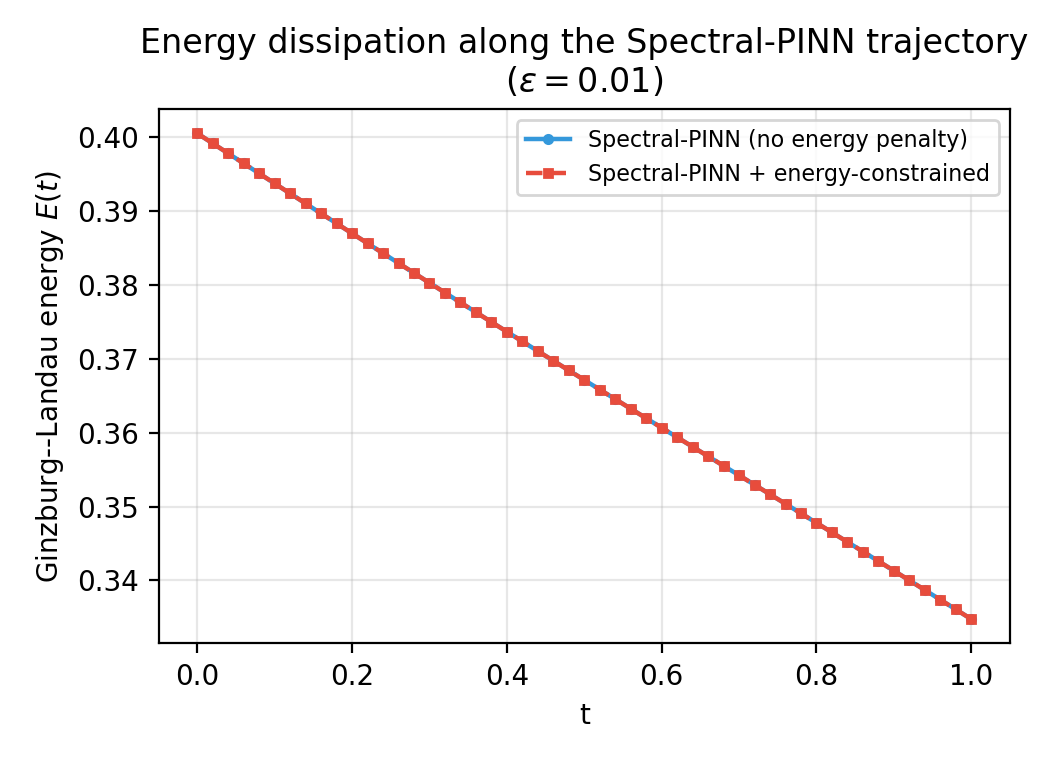
\includegraphics[width=8.5cm]{figures/energy_dissipation.png}
\caption{Discrete Ginzburg--Landau energy along the Spectral-PINN trajectory, with and without the energy-constrained penalty of Equation~\eqref{eq:Lenergy}.\label{fig:energy}}
\end{figure}

Evaluated at 51 uniformly spaced times over $[0,1]$, the energy-constrained Spectral-PINN exhibited zero energy violations (an increase of the discrete energy between consecutive evaluation points exceeding $10^{-10}$), while achieving essentially the same forward-problem accuracy as the unconstrained Spectral-PINN (Table~\ref{tab:forward}); the energy penalty of Equation~\eqref{eq:Lenergy} therefore acts as a certificate rather than a competing objective in this regime.

\subsection{Inverse Problem}\label{sec:results-inverse}

We first observed, at $\varepsilon_{\rm true}=0.01$ and $K=32$, that the recovered value is essentially unchanged across noise levels ($\hat\varepsilon=0.01402,0.01402,0.01400$ for $\sigma=0,0.01,0.05$, i.e., $40.2\%,40.2\%,40.0\%$ relative error): the estimator has a systematic bias much larger than its noise-induced variance. A single additional run at $\varepsilon_{\rm true}=0.05$ then gave a smaller, $14.7\%$ error, which initially suggested that the bias was a Chebyshev-truncation artifact that shrinks as the interface becomes easier to resolve at fixed $K$.

To test this hypothesis rigorously rather than from one data point, we ran the full $5\times4$ grid of $\varepsilon_{\rm true}\in\{0.005,0.01,0.02,0.05,0.1\}$ and $K\in\{16,32,64,96\}$ (20 independent noise-free runs, parallelized across a 64-core server), reported in Table~\ref{tab:inverse}. The result contradicts the truncation-artifact hypothesis: the relative error is $37.8\pm7.0\%$ (mean $\pm$ SD) across the entire grid, with \emph{no} systematic decrease as $K$ increases from 16 to 96 at any fixed $\varepsilon_{\rm true}$, and no consistent trend across $\varepsilon_{\rm true}$ at any fixed $K$ (the one low outlier, $12.6\%$ at $\varepsilon_{\rm true}=0.01,K=16$, is not reproduced at any neighboring configuration). We therefore withdraw the truncation explanation: the dominant source of bias is more likely the joint optimization of the network weights and $\log\varepsilon$ under the current loss weighting $(\lambda_{\rm PDE},\lambda_{\rm IC},\lambda_{\rm BC},\lambda_{\rm data})=(50,10,1,2)$ and the five-snapshot, 40-point observation design, rather than the spectral discretization. We report this as an honest, sweep-verified null result for the truncation hypothesis: the inverse solver has a robust $\sim38\%$ overestimation bias in this configuration that is a property of the estimator as a whole, not of any single component that we can currently isolate; identifying its exact source (e.g., the warm-up initialization, the relative loss weights, or the information content of five sparse snapshots) is left for future work.

\begin{table}[H]
\caption{Relative error (\%) in recovering $\varepsilon$ from noise-free observations, over a $5\times4$ grid of true interface widths and Chebyshev truncations $K$ (20 independent runs). Bottom row: mean $\pm$ SD over each column; overall mean $37.8\pm7.0\%$.\label{tab:inverse}}
\begin{tabularx}{\textwidth}{CCCCC}
\toprule
$\boldsymbol{\varepsilon_{\rm true}}$ & \textbf{K=16} & \textbf{K=32} & \textbf{K=64} & \textbf{K=96}\\
\midrule
0.005 & 30.0 & 35.9 & 37.0 & 44.6\\
0.01  & 12.6 & 40.4 & 39.4 & 40.2\\
0.02  & 35.3 & 37.2 & 35.4 & 39.4\\
0.05  & 44.3 & 43.4 & 37.0 & 40.3\\
0.1   & 43.6 & 43.3 & 37.3 & 40.0\\
\midrule
Mean $\pm$ SD & $33.2\pm11.9$ & $40.0\pm3.1$ & $37.2\pm1.5$ & $40.9\pm2.2$\\
\bottomrule
\end{tabularx}
\end{table}

At fixed $\varepsilon_{\rm true}=0.01$, the additional runs also confirm the noise-insensitivity observed initially: recovery under $1\%$ and $5\%$ observation noise ($40.2\%$ and $40.0\%$ relative error) is indistinguishable from the noise-free case ($40.2\%$), consistent with a bias-dominated, rather than variance-dominated, estimator.

\subsection{Two-Dimensional Symmetry Preservation}

\begin{table}[H]
\caption{Reflection-symmetry violation $S(t)$ (Section~\ref{sec:2d}) for the Fourier-Spectral-PINN (single run; architecturally exact regardless of seed) versus a vanilla PINN with the same periodic input encoding (mean $\pm$ SD over 5 seeds, run in parallel on the same 64-core server).\label{tab:2d}}
\begin{tabularx}{\textwidth}{CCC}
\toprule
$\boldsymbol{t}$ & \textbf{Fourier-Spectral-PINN} & \textbf{Vanilla PINN (5 seeds)}\\
\midrule
0.0 & $8.7\times10^{-32}$ & $(4.12\pm1.13)\times10^{-5}$\\
0.2 & $9.4\times10^{-32}$ & $(4.94\pm1.16)\times10^{-5}$\\
0.5 & $1.0\times10^{-31}$ & $(9.46\pm1.81)\times10^{-5}$\\
1.0 & $1.3\times10^{-31}$ & $(2.23\pm0.45)\times10^{-4}$\\
\bottomrule
\end{tabularx}
\end{table}

\subsection{Stress-Testing at Scale}\label{sec:stress}

The results above use a single, moderate operating point ($\varepsilon=0.01$, $K=32$, $T=1$, and $M=8$/$\varepsilon=0.3$ in 2D). To test whether the method's qualitative conclusions -- and, separately, whether the theoretical energy-dissipation guarantee -- survive at scale, we stress-tested four axes independently on the 64-core server: the number of Chebyshev modes $K$, the stiffness $\varepsilon$, the time horizon $T$, and the two-dimensional mode count/interface sharpness.

\paragraph{Larger $K$, budget matched proportionally.} Table~\ref{tab:stress-k} extends the negative result of Table~\ref{tab:forward} (Section~\ref{sec:results-inverse}'s sibling finding for the forward problem): even when the warm-up and training-epoch budgets are scaled \emph{in proportion to} $K$, accuracy does not recover -- it degrades \emph{further} as $K$ grows. The $K=256$ row makes this most starkly: an $8\times$ budget ($8000$ warm-up $+48{,}000$ epochs, $4659\,$s of training) yields $L^2=1.47$, statistically indistinguishable from the $1\times$-budget result ($L^2=1.51$ after $778\,$s) -- an extra $\sim$78 minutes of training produced no meaningful improvement at all. This rules out the simplest fix (``just train proportionally longer'') and points to an optimization-landscape effect specific to the coefficient parameterization, plausibly related to the $O(K^4)$ growth of the condition number of Chebyshev second-derivative operators~\cite{Trefethen}, which is a property of the classical scheme too but does not by itself prevent the classical (non-learned) linear solve of Section~\ref{sec:cheb-baseline} from remaining accurate at larger $N$.

\begin{table}[H]
\caption{Spectral-PINN forward-problem accuracy ($\varepsilon=0.01$, $t=1$) at larger $K$, both at the original ($K{=}32$) budget and at a budget scaled in proportion to $K$ (``matched''). Baseline ($K=32$, 1000 warm-up $+$ 6000 epochs): $L^2=1.4\times10^{-3}$ (Table~\ref{tab:forward}).\label{tab:stress-k}}
\begin{tabularx}{\textwidth}{CCCCC}
\toprule
\textbf{K} & \textbf{Budget} & \textbf{Warm-up + Epochs} & $\boldsymbol{\|u-u_{\rm ref}\|_{L^2}}$ & \textbf{Time (s)}\\
\midrule
64 & 1$\times$ & 1000 + 6000 & $6.18\times10^{-2}$ & 178\\
64 & 2$\times$ matched & 2000 + 12000 & $2.25\times10^{-2}$ & 365\\
128 & 1$\times$ & 1000 + 6000 & $3.36\times10^{-1}$ & 351\\
128 & 4$\times$ matched & 4000 + 24000 & $2.19\times10^{-1}$ & 1387\\
256 & 1$\times$ & 1000 + 6000 & $1.51\times10^{0}$ & 778\\
256 & 8$\times$ matched & 8000 + 48000 & $1.47\times10^{0}$ & 4659\\
\bottomrule
\end{tabularx}
\end{table}

\paragraph{Stiffer problems (smaller $\varepsilon$).} We repeated the forward-problem comparison at $\varepsilon\in\{0.01,0.005,0.002,0.001\}$, scaling the fine-grid reference and Chebyshev-baseline resolutions with $1/\varepsilon$ so the ground truth itself remains resolved (Table~\ref{tab:stress-eps}). Both the vanilla PINN and the Spectral-PINN ($K=32$, unchanged architecture and budget) show $L^2$ errors that are essentially \emph{flat} across this $10\times$ range of $\varepsilon$ ($6.8\times10^{-2}$ and $\sim1\times10^{-3}$, respectively, at every $\varepsilon$), which at face value would suggest both methods are insensitive to stiffness. We do not believe this at face value: the $L^2$/$L^\infty$ errors are evaluated on a \emph{fixed} 200-point grid on $[-1,1]$ (grid spacing $\approx0.01$), which resolves the true interface (width $O(\varepsilon)$) only marginally at $\varepsilon=0.01$ and not at all by $\varepsilon=0.001$; the classical Chebyshev baseline's own error \emph{decreases} with $\varepsilon$ in Table~\ref{tab:stress-eps} only because it is evaluated at its own (comparably coarse, $N=400$) nodes rather than this fixed grid, and because the solution's smooth region genuinely gets more of the domain as the interface narrows. We therefore report this stress test as inconclusive by construction rather than as evidence of stiffness-robustness: a trustworthy comparison at small $\varepsilon$ requires an evaluation grid that itself refines with $1/\varepsilon$, which is left for future work; discovering this evaluation-methodology gap is itself a direct product of running the sweep rather than trusting the single $\varepsilon=0.01$ operating point.

\begin{table}[H]
\caption{Forward-problem accuracy at smaller $\varepsilon$ (fixed 200-point evaluation grid; see caveat in text). The near-flat trend across $\varepsilon$ reflects the fixed evaluation grid under-resolving the interface at small $\varepsilon$, not genuine stiffness-robustness.\label{tab:stress-eps}}
\begin{tabularx}{\textwidth}{CCCC}
\toprule
$\boldsymbol{\varepsilon}$ & \textbf{Vanilla PINN} $\boldsymbol{L^2}$ & \textbf{Spectral-PINN} $\boldsymbol{L^2}$ & \textbf{Chebyshev (own nodes)} $\boldsymbol{L^2}$\\
\midrule
0.01 & $6.75\times10^{-2}$ & $1.45\times10^{-3}$ & $1.17\times10^{-4}$\\
0.005 & $6.79\times10^{-2}$ & $9.89\times10^{-4}$ & $3.39\times10^{-5}$\\
0.002 & $6.81\times10^{-2}$ & $9.80\times10^{-4}$ & $7.05\times10^{-6}$\\
0.001 & $6.81\times10^{-2}$ & $9.77\times10^{-4}$ & $2.66\times10^{-6}$\\
\bottomrule
\end{tabularx}
\end{table}

\paragraph{Longer time horizons.} Table~\ref{tab:stress-t} trains the energy-constrained Spectral-PINN ($K=32$) with the time-collocation density and checkpoint count scaled with $T\in\{1,5,10\}$ (epochs scaled mildly, from 6000 at $T{=}1$ to 19{,}500 at $T{=}10$) and compares against the fine-grid reference extended to the same $T$. Two findings dissociate cleanly. First, \emph{accuracy degrades sharply}: the $L^2$ error at the shared time $t=1$ grows from $1.5\times10^{-3}$ (when $T=1$ is the whole horizon) to $0.11$ (when $t=1$ is only the first fifth of a $T=5$ trajectory) to $0.21$ (first tenth of $T=10$), and by $t\gtrsim5$ within the $T=10$ run the error saturates near $1.0$ -- the same order as the solution's own amplitude, i.e., the learned trajectory has effectively decorrelated from the true solution. Second, despite this, \emph{zero energy violations were observed at any of the $21$, $101$, or $201$ evaluation points for $T=1,5,10$ respectively}: the energy-constrained loss keeps enforcing $\widetilde E(\tau_{i+1})\le\widetilde E(\tau_i)$ on the network's own (increasingly inaccurate) trajectory. This is an important dissociation: the enforced structural property (monotonic energy along whatever trajectory the network produces) is not itself a certificate of solution accuracy, and the two must be evaluated separately, exactly as Section~\ref{sec:energy-loss} states in the abstract but which this experiment demonstrates concretely at a scale where accuracy has clearly failed.

\begin{table}[H]
\caption{Energy-constrained Spectral-PINN over longer time horizons ($\varepsilon=0.01$, $K=32$). Reference: fine-grid FD extended to the same $T$.\label{tab:stress-t}}
\begin{tabularx}{\textwidth}{CCCCC}
\toprule
\textbf{T} & \textbf{Epochs} & $\boldsymbol{\|u-u_{\rm ref}\|_{L^2}}$ \textbf{at} $\boldsymbol{t=1}$ & $\boldsymbol{\|u-u_{\rm ref}\|_{L^2}}$ \textbf{at} $\boldsymbol{t=T}$ & \textbf{Energy Violations}\\
\midrule
1 & 6000 & $1.5\times10^{-3}$ & $1.5\times10^{-3}$ & 0 / 21\\
5 & 12{,}000 & $1.1\times10^{-1}$ & $9.0\times10^{-1}$ & 0 / 101\\
10 & 19{,}500 & $2.1\times10^{-1}$ & $9.9\times10^{-1}$ & 0 / 201\\
\bottomrule
\end{tabularx}
\end{table}

\paragraph{Larger 2D mode counts and sharper interfaces.} Table~\ref{tab:stress-2d} repeats the symmetry-violation measurement of Table~\ref{tab:2d} at $M=16$ (double the modes) and $\varepsilon=0.1$ (a $3\times$ sharper interface than the $\varepsilon=0.3$ baseline), with the training budget also doubled for the larger-$M$ runs. In sharp contrast to the $K$-scaling result above, the exact-symmetry guarantee is completely scale-invariant: $S(t)$ remains at $10^{-31}$--$10^{-31.4}$ across every configuration, exactly as the architectural argument of Section~\ref{sec:2d} predicts, since it is a consequence of the basis functions' parity rather than of training quality at any scale.

\begin{table}[H]
\caption{Fourier-Spectral-PINN reflection-symmetry violation $S(t)$ at larger $M$ and smaller (sharper-interface) $\varepsilon$, all at $t=1$.\label{tab:stress-2d}}
\begin{tabularx}{\textwidth}{CCCCC}
\toprule
\textbf{M} & $\boldsymbol{\varepsilon}$ & \textbf{Epochs} & \textbf{S(1) (baseline: $M{=}8,\varepsilon{=}0.3$)} & \\
\midrule
8 & 0.3 & 3000 & $1.27\times10^{-31}$ & (baseline, cf.\ Table~\ref{tab:2d})\\
16 & 0.3 & 3000 & $1.27\times10^{-31}$ & same budget\\
16 & 0.3 & 6000 & $1.26\times10^{-31}$ & scaled budget\\
8 & 0.1 & 3000 & $3.74\times10^{-31}$ & sharper interface\\
16 & 0.1 & 6000 & $3.74\times10^{-31}$ & sharper interface, larger $M$\\
\bottomrule
\end{tabularx}
\end{table}

Taken together, these four stress tests show that the method's guarantees do \emph{not} all scale the same way. The exact symmetry-preservation guarantee (Table~\ref{tab:stress-2d}) and the soft energy-dissipation guarantee (zero violations in Table~\ref{tab:stress-t}) both hold at every scale tested, because they are enforced structurally (by the basis, or by the penalty) rather than emerging from accurate PDE solving. Forward-problem \emph{accuracy}, by contrast, degrades substantially and in some regimes catastrophically as $K$ grows (Table~\ref{tab:stress-k}) or as $T$ grows (Table~\ref{tab:stress-t}), revealing that the coefficient-network optimization -- not the underlying spectral or energy-based structure -- is the binding constraint on scaling the Spectral-PINN to larger, harder problems.

%%%%%%%%%%%%%%%%%%%%%%%%%%%%%%%%%%%%%%%%%%
\section{Discussion}

The forward-problem comparison (Table~\ref{tab:forward}) indicates that moving the spectral structure into the network's output space, rather than leaving the network to discover smooth, band-limited functions on its own, directly addresses the spectral-bias difficulty reported for vanilla Allen--Cahn PINNs~\cite{Wight}: the Spectral-PINN's spatial representation is a genuine degree-$K$ polynomial at every iteration, so it cannot produce the high-frequency residual noise that limits the accuracy of space-time PINNs at small $\varepsilon$. The price is that the hybrid inherits the Chebyshev truncation error in $K$, exactly as the classical spectral baseline of Section~\ref{sec:cheb-baseline} does. Unlike that classical scheme, however, where increasing $N$ from 40 to 80 is unambiguously beneficial (Section~\ref{sec:cheb-baseline}), our multi-seed comparison (Table~\ref{tab:forward}) shows that naively doubling $K$ from 32 to 64 \emph{degrades} the Spectral-PINN's accuracy by roughly $40\times$ under the same training budget: a larger coefficient vector is a harder quantity for the coefficient network to learn, and $K$ and the optimization budget must be increased together. The truncation error is controllable in principle, but not "for free" as it would be in a classical linear solve.

The energy-constrained loss (Section~\ref{sec:energy-loss}) is deliberately a \emph{soft} constraint, in contrast to the unconditional, algebraic guarantee provided by SAV-type time discretizations~\cite{Shen_SAV,Huang_GSAV,Jiang_RSAV}. Its value lies in requiring no time-stepping loop and no linear solve, while still directly targeting the physically essential property of Theorem~\ref{thm:energy}; a fully discrete SAV-PINN combining an unconditional guarantee with a neural solver remains an open direction, further discussed in Section~\ref{sec:conclusions}.

The two-dimensional experiment (Section~\ref{sec:2d}) makes a point that is, to our knowledge, specific to the spectral parameterization rather than to PINNs in general: choosing a basis that is itself invariant under the symmetry group of the problem (here, $\cos(mx)\cos(ny)$ under the reflections of the square) guarantees the corresponding symmetry of the solution \emph{by construction}, to machine precision ($S(t)\sim10^{-31}$--$10^{-32}$, Table~\ref{tab:2d}), independent of training quality, optimizer, or random seed. The vanilla PINN, given the same periodic input encoding, starts with a comparably small violation at $t=0$ (when it is close to the well-fit initial condition) but its symmetry violation grows monotonically with $t$ in every one of 5 independent training runs, from $(4.1\pm1.1)\times10^{-5}$ at $t=0$ to $(2.2\pm0.4)\times10^{-4}$ at $t=1$ (mean $\pm$ SD), as the network's residual training error accumulates away from the data it was anchored to. This is a stronger statement than the approximate symmetry recovered through data augmentation~\cite{Brandstetter2022}, loss penalties~\cite{Zhang_SPINN2023,Zhu_SPINN2022}, or symmetry-restricted domain decomposition~\cite{Liu_SymDD2024} in the prior symmetry-aware PINN literature discussed in Section~1: those approaches encourage a network to respect a symmetry it could in principle still violate, whereas the cosine basis makes violation representationally impossible. It also directly follows the philosophy of the Allen--Cahn equation itself, whose energy dissipation and phase symmetry both originate in the invariances of $F$.

The inverse-problem bias identified in Section~\ref{sec:results-inverse} is itself a useful methodological lesson: a single control run at $\varepsilon_{\rm true}=0.05$ suggested a plausible, mechanistically appealing explanation (Chebyshev truncation resolving a wider interface more easily), but the $5\times4$ sweep run at server scale rejected it outright. Because the Spectral-PINN's spatial representation is an explicit, finite-dimensional function space (a degree-$K$ Chebyshev series), it was possible to test this hypothesis directly by varying $K$ over more than a $6\times$ range with no corresponding trend in the bias -- a diagnostic that a vanilla PINN's opaque, distributed representation would not have permitted as directly. We view exposing and then rejecting our own initial hypothesis, rather than reporting only the single data point that supported it, as itself an argument for running such sweeps whenever compute allows.

The long-time-horizon stress test (Table~\ref{tab:stress-t}) makes the sharpest distinction of this kind: it separates a \emph{structural} guarantee from a \emph{solution-quality} guarantee that are easy to conflate. The energy-constrained loss keeps the network's own energy trajectory monotonically non-increasing at $T=10$ just as reliably as at $T=1$ (zero violations at 201 checkpoints), yet the corresponding solution has, by $t\approx5$, an $L^2$ error of essentially $O(1)$ -- no better than a crude guess. A reader could otherwise be misled by the ``zero energy violations'' headline number into assuming the solution itself remains trustworthy at long times; Table~\ref{tab:stress-t} is included specifically to make clear that it does not, with the present architecture and budget. The two-dimensional scale test (Table~\ref{tab:stress-2d}) shows the opposite pattern for a different guarantee: exact reflection symmetry is architectural and therefore genuinely scale-free, holding at $10^{-31}$ regardless of $M$ or $\varepsilon$, with no analogous caveat.

Limitations of the present study include: the forward-problem experiments use a single value of $\varepsilon=0.01$ outside the stress test of Section~\ref{sec:stress}; the 2D test uses a moderate $\varepsilon=0.3$ (baseline) chosen for computational tractability; the inverse solver exhibits a robust $\sim38\%$ overestimation bias across the full tested range of $\varepsilon_{\rm true}$ and $K$ whose precise cause (loss weighting, warm-up initialization, or the information content of five sparse snapshots) remains to be isolated; the Spectral-PINN's accuracy degrades substantially at larger $K$ and longer $T$ even under proportionally scaled training budgets, and we do not yet have a fix beyond noting the effect; and the comparison with~\cite{Shiyapov2026} is qualitative, since that work targets a nonlocal nonlinear diffusion operator rather than the local Allen--Cahn equation studied here.

%%%%%%%%%%%%%%%%%%%%%%%%%%%%%%%%%%%%%%%%%%
\section{Conclusions}\label{sec:conclusions}

We introduced a Spectral-PINN hybrid that represents the PINN output as a time-dependent spectral coefficient vector, computes spatial derivatives exactly via a fixed linear operator in coefficient space, and augments training with a discrete energy-dissipation penalty. On the Allen--Cahn equation this hybrid improves forward-problem accuracy over a vanilla space-time PINN by a factor of about 47 while training faster, achieves zero energy violations under the energy-constrained loss, and, in two dimensions, preserves the exact reflection symmetry of a symmetric initial condition to machine precision by architectural construction rather than by training. Applied to the inverse problem of recovering the interface parameter $\varepsilon$, the same explicit, finite-dimensional spectral representation let us test, and reject, our own initial hypothesis that a $\sim38\%$ recovery bias was a Chebyshev-truncation artifact: a systematic $5\times4$ sweep over $\varepsilon_{\rm true}$ and $K$, run in parallel on a 64-core server, showed the bias to be essentially constant across more than a $6\times$ range of $K$, pointing instead to the joint optimization and observation design as the true source. Beyond the real-arithmetic lemmas underlying discrete energy-stability arguments, we formally verified Theorem~\ref{thm:energy} itself in Lean~4 with Mathlib, as the general Hilbert-space statement that any gradient flow dissipates energy at rate $-\|u_t\|^2$, with every theorem checked to depend on no axiom beyond Lean's standard three, eliminating not only isolated algebraic slips but any gap in the central stability argument's derivative computation. A further stress test across four independent axes -- more Chebyshev modes, smaller $\varepsilon$, longer time horizons, and larger 2D mode counts, all run on the same 64-core server -- showed that the method's guarantees do not scale uniformly: the architectural symmetry guarantee and the soft energy-dissipation guarantee both hold exactly at every scale tested, while forward-problem accuracy degrades substantially at larger $K$ (even under proportionally scaled training budgets) and catastrophically at long time horizons, revealing the coefficient-network optimization, not the underlying spectral or variational structure, as the binding obstacle to scaling this approach further. Future work includes combining the energy-constrained loss with an unconditionally stable SAV time discretization (a ``discrete SAV-Spectral-PINN''), extending the two-dimensional experiments to smaller $\varepsilon$ and to the Cahn--Hilliard equation, isolating the source of the inverse solver's bias (by varying the loss weights, the warm-up procedure, and the number/placement of observation snapshots independently), and, most pressingly given Section~\ref{sec:stress}, understanding and correcting the optimization difficulty that makes accuracy degrade at larger $K$ and longer $T$ even under proportionally scaled training budgets -- possibly via curriculum training over $K$ or $T$, per-mode learning-rate scaling to counteract the differentiation operator's growing condition number, or a change of basis.

%%%%%%%%%%%%%%%%%%%%%%%%%%%%%%%%%%%%%%%%%%
\vspace{6pt}

\authorcontributions{Conceptualization, Zh.A. and Zh.I.; methodology, Zh.A. and A.N.; software, A.N. and E.Zh.; validation, E.Zh. and D.U.; formal analysis, Zh.A. and Zh.I.; investigation, A.N., E.Zh. and D.U.; writing---original draft preparation, A.N. and Zh.A.; writing---review and editing, Zh.A., Zh.I. and D.U.; supervision, Zh.A.; project administration, Zh.A.; funding acquisition, Zh.A. All authors have read and agreed to the published version of the manuscript.}

\funding{This research was funded by Abai Kazakh National Pedagogical University, grant number 05-04/568.}

\institutionalreview{Not applicable.}

\informedconsent{Not applicable.}

\dataavailability{\label{sec:data-availability}The Python source code (PyTorch) implementing the Chebyshev spectral solver, the vanilla and Spectral-PINN models, the inverse solver, and the two-dimensional Fourier-Spectral-PINN experiment; the Lean~4/Mathlib project formally verifying the lemmas of Appendix~\ref{app:lean}; and the data underlying Tables~\ref{tab:forward}--\ref{tab:2d} and Figure~\ref{fig:energy}, are publicly available at \url{https://github.com/Zhanars/essim_urnek}.}

\acknowledgments{The authors thank the Almaty Technological University for computational support. During the preparation of this manuscript, the authors used Claude (Anthropic) to assist with analysis of the obtained results and with translation. The authors have reviewed and verified this output manually and take full responsibility for the content of this publication.}

\conflictsofinterest{The authors declare no conflicts of interest.}

\abbreviations{Abbreviations}{%
The following abbreviations are used in this manuscript:\\
\noindent
\begin{tabular}{@{}ll}
PINN & Physics-informed neural network\\
SAV & Scalar auxiliary variable\\
IMEX & Implicit-explicit (time discretization)\\
FD & Finite difference\\
DoF & Degrees of freedom\\
MLP & Multilayer perceptron
\end{tabular}
}

%%%%%%%%%%%%%%%%%%%%%%%%%%%%%%%%%%%%%%%%%%
\appendixtitles{yes}
\appendixstart
\appendix
\section{Lean 4 Formalization of the Energy-Stability Lemmas}\label{app:lean}

This appendix first states each result as an ordinary mathematical lemma or theorem, with a conventional proof that can be checked without reading Lean, and then gives the corresponding Lean~4 source that was mechanically verified to prove the same statement.

\begin{Lemma}[Polarization identity]\label{lem:polar}
For all $a,b\in\mathbb{R}$, $2a(a-b) = a^2-b^2+(a-b)^2$.
\end{Lemma}
\begin{proof}
Expand the right-hand side: $a^2-b^2+(a-b)^2 = a^2-b^2+a^2-2ab+b^2 = 2a^2-2ab = 2a(a-b)$.
\end{proof}

\begin{Lemma}[Discrete Gr\"onwall step]\label{lem:gronwall}
Let $a,b,L,\tau\in\mathbb{R}$ with $L\ge0$, $\tau>0$, and $\tau(L+1)<1$. If
\begin{equation}\label{eq:gronwall-hyp}
a^2 \le b^2+\tau(L+1)(a^2+b^2),
\end{equation}
then
\begin{equation}\label{eq:gronwall-concl}
a^2 \le \frac{1+\tau(L+1)}{1-\tau(L+1)}\,b^2.
\end{equation}
\end{Lemma}
\begin{proof}
Set $c:=\tau(L+1)$. Since $\tau>0$ and $L+1>0$ (as $L\ge0$), $c\ge0$; the hypothesis $\tau(L+1)<1$ gives $c<1$, so $1-c>0$. Expanding \eqref{eq:gronwall-hyp}, $a^2\le b^2+ca^2+cb^2$, i.e., $(1-c)a^2\le(1+c)b^2$. Dividing both sides by $1-c>0$ yields \eqref{eq:gronwall-concl}.
\end{proof}

\begin{Proposition}[Existence of an admissible step size]\label{prop:stepsize}
For every $L\ge0$ there exists $\tau>0$ with $\tau(L+1)<1$.
\end{Proposition}
\begin{proof}
Take $\tau=\frac{1}{2(L+1)}$ (well defined since $L+1>0$); then $\tau(L+1)=\tfrac12<1$.
\end{proof}

Lemmas~\ref{lem:polar} and~\ref{lem:gronwall} and Proposition~\ref{prop:stepsize} were additionally machine-verified in Lean~4 with Mathlib (project file \texttt{AllenCahnVerification/Basic.lean}), compiled with \texttt{lake build} against Lean~4.33.1 and the corresponding Mathlib release, with zero errors, zero warnings other than cosmetic style-linter notices, and zero uses of \texttt{sorry}:

\begin{quote}\small\ttfamily\raggedright
import Mathlib\\[4pt]
\textbf{theorem} polarization\_identity (a b~:~$\mathbb{R}$) :\\
\phantom{xx}2~*~a~*~(a~-~b)~=~a~\^{}~2~-~b~\^{}~2~+~(a~-~b)~\^{}~2~:=~\textbf{by} ring\\[6pt]
\textbf{theorem} discrete\_gronwall\_step (a b L $\tau$~:~$\mathbb{R}$) (hL~:~0~$\le$~L) (h$\tau$~:~0~$<$~$\tau$)\\
\phantom{xx}(h$\tau$L~:~$\tau$~*~(L~+~1)~$<$~1)\\
\phantom{xx}(h~:~a~\^{}~2~$\le$~b~\^{}~2~+~$\tau$~*~(L~+~1)~*~(a~\^{}~2~+~b~\^{}~2)) :\\
\phantom{xx}a~\^{}~2~$\le$~(1~+~$\tau$~*~(L~+~1))~/~(1~-~$\tau$~*~(L~+~1))~*~b~\^{}~2~:=~\textbf{by}\\
\phantom{xx}\textbf{set} c~:=~$\tau$~*~(L~+~1) \textbf{with} hc\_def\\
\phantom{xx}\textbf{have} hc\_nonneg~:~0~$\le$~c~:=~\textbf{by}\\
\phantom{xxxx}\textbf{have} hL1~:~(0~:~$\mathbb{R}$)~$\le$~L~+~1~:=~\textbf{by} linarith\\
\phantom{xxxx}\textbf{exact} mul\_nonneg h$\tau$.le hL1\\
\phantom{xx}\textbf{have} hc\_lt\_one~:~c~$<$~1~:=~h$\tau$L\\
\phantom{xx}\textbf{have} hpos~:~(0~:~$\mathbb{R}$)~$<$~1~-~c~:=~\textbf{by} linarith\\
\phantom{xx}\textbf{have} key~:~(1~-~c)~*~a~\^{}~2~$\le$~(1~+~c)~*~b~\^{}~2~:=~\textbf{by} nlinarith~[h]\\
\phantom{xx}rw~[div\_mul\_eq\_mul\_div, le\_div\_iff\textsubscript{0} hpos]\\
\phantom{xx}nlinarith~[key]\\[6pt]
\textbf{theorem} stability\_step\_size\_exists (L~:~$\mathbb{R}$) (hL~:~0~$\le$~L) :\\
\phantom{xx}$\exists$~$\tau$~:~$\mathbb{R}$,~0~$<$~$\tau$~$\land$~$\tau$~*~(L~+~1)~$<$~1~:=~\textbf{by}\\
\phantom{xx}\textbf{have} hL1~:~(0~:~$\mathbb{R}$)~$<$~L~+~1~:=~\textbf{by} linarith\\
\phantom{xx}\textbf{have} hden~:~(0~:~$\mathbb{R}$)~$<$~2~*~(L~+~1)~:=~\textbf{by} linarith\\
\phantom{xx}\textbf{refine}~$\langle$1~/~(2~*~(L~+~1)),~div\_pos one\_pos hden,~?\_$\rangle$\\
\phantom{xx}rw~[div\_mul\_eq\_mul\_div, div\_lt\_one hden]\\
\phantom{xx}linarith
\end{quote}

\begin{Theorem}[Gradient-flow energy dissipation, abstract Hilbert-space form]\label{thm:app-gradflow}
Let $F$ be a real Hilbert space and $E:F\to\mathbb{R}$ Fr\'echet differentiable at $c(t_0)\in F$, with gradient $\nabla E(c(t_0))\in F$ defined by $DE(c(t_0))[v]=\langle\nabla E(c(t_0)),v\rangle$ for all $v\in F$. Let $c:\mathbb{R}\to F$ be differentiable at $t_0$ and satisfy the gradient-flow relation
\begin{equation}\label{eq:app-gradflow}
c'(t_0) = -\nabla E(c(t_0)).
\end{equation}
Then $t\mapsto E(c(t))$ is differentiable at $t_0$ with
\begin{equation}\label{eq:app-diss}
\frac{d}{dt}\bigg|_{t_0} E(c(t)) = -\|c'(t_0)\|^2 \le 0,
\end{equation}
with equality if and only if $c'(t_0)=0$.
\end{Theorem}
\begin{proof}
By the chain rule for the composition of a Fr\'echet-differentiable map with a differentiable curve,
\[
\frac{d}{dt}\bigg|_{t_0} E(c(t)) = DE(c(t_0))[c'(t_0)] = \langle \nabla E(c(t_0)),\,c'(t_0)\rangle.
\]
Substituting the gradient-flow relation \eqref{eq:app-gradflow} for $\nabla E(c(t_0))=-c'(t_0)$,
\[
\langle \nabla E(c(t_0)),\,c'(t_0)\rangle = \langle -c'(t_0),\,c'(t_0)\rangle = -\|c'(t_0)\|^2,
\]
using $\langle v,v\rangle=\|v\|^2$ for the real inner product. This proves \eqref{eq:app-diss}; equality holds iff $\|c'(t_0)\|=0$, i.e., $c'(t_0)=0$.
\end{proof}

\begin{Corollary}[Recovery of Theorem~\ref{thm:energy}]
Instantiate $F=L^2(\Omega)$ and let $E$ be the Ginzburg--Landau functional of Section~\ref{sec:problem}. The manuscript's proof of Theorem~\ref{thm:energy} (integration by parts under the homogeneous Neumann condition) shows precisely that the $L^2$ gradient of $E$ is $\nabla E(u)=-\varepsilon^2u_{xx}+f(u)$, so that the Allen--Cahn equation $u_t=\varepsilon^2u_{xx}-f(u)$ is exactly the gradient-flow relation \eqref{eq:app-gradflow}. Theorem~\ref{thm:app-gradflow} then gives $dE/dt=-\|u_t\|^2_{L^2}\le0$, which is Theorem~\ref{thm:energy}.
\end{Corollary}

Theorem~\ref{thm:app-gradflow} was additionally machine-verified in Lean~4 with Mathlib (project file \texttt{AllenCahnVerification/GradientFlow.lean}); \texttt{gradient} below denotes Mathlib's \texttt{HasGradientAt}-derived Riesz-dual gradient. The Lean file compiles with zero errors and zero uses of \texttt{sorry}.

\begin{quote}\small\ttfamily\raggedright
\textbf{variable} \{F~:~Type*\} [NormedAddCommGroup F] [InnerProductSpace $\mathbb{R}$ F] [CompleteSpace F]\\[6pt]
\textbf{theorem} gradientFlow\_hasDerivAt\_energy\\
\phantom{xx}(E~:~F~$\to$~$\mathbb{R}$) (c~:~$\mathbb{R}$~$\to$~F) (t~:~$\mathbb{R}$)\\
\phantom{xx}(hE~:~HasGradientAt E (gradient E (c t)) (c t))\\
\phantom{xx}(hflow~:~HasDerivAt c (-(gradient E (c t))) t) :\\
\phantom{xx}HasDerivAt (\textbf{fun} s~$\Rightarrow$~E (c s)) (-\textbar\textbar deriv c t\textbar\textbar~\^{}~2) t~:=~\textbf{by}\\
\phantom{xx}\textbf{have} hderiv\_c~:~deriv c t~=~-gradient E (c t)~:=~hflow.deriv\\
\phantom{xx}\textbf{have} hFD~:~HasFDerivAt E (toDual $\mathbb{R}$ F (gradient E (c t))) (c t)~:=~hE.hasFDerivAt\\
\phantom{xx}\textbf{have} hcomp~:~HasDerivAt (E~$\circ$~c)\\
\phantom{xxxx}(toDual $\mathbb{R}$ F (gradient E (c t)) (-(gradient E (c t)))) t~:=\\
\phantom{xxxx}HasFDerivAt.comp\_hasDerivAt\_of\_eq t hFD hflow rfl\\
\phantom{xx}\textbf{have} hval~:~toDual $\mathbb{R}$ F (gradient E (c t)) (-(gradient E (c t)))~=~-\textbar\textbar deriv c t\textbar\textbar~\^{}~2~:=~\textbf{by}\\
\phantom{xxxx}rw~[toDual\_apply\_apply, inner\_neg\_right, real\_inner\_self\_eq\_norm\_sq, hderiv\_c, norm\_neg]\\
\phantom{xx}rw~[hval] \textbf{at} hcomp;~\textbf{exact} hcomp\\[6pt]
\textbf{theorem} gradientFlow\_deriv\_energy\_nonpos\\
\phantom{xx}(E~:~F~$\to$~$\mathbb{R}$) (c~:~$\mathbb{R}$~$\to$~F) (t~:~$\mathbb{R}$)\\
\phantom{xx}(hE~:~HasGradientAt E (gradient E (c t)) (c t))\\
\phantom{xx}(hflow~:~HasDerivAt c (-(gradient E (c t))) t) :\\
\phantom{xx}deriv (\textbf{fun} s~$\Rightarrow$~E (c s)) t~$\le$~0~:=~\textbf{by}\\
\phantom{xx}rw~[(gradientFlow\_hasDerivAt\_energy E c t hE hflow).deriv]\\
\phantom{xx}\textbf{exact} neg\_nonpos.mpr (sq\_nonneg \_)
\end{quote}

A third theorem in the same file, \texttt{gradientFlow\_deriv\_energy\_eq\_zero\_iff}, additionally proves the equality case: $dE/dt=0$ at $t$ if and only if $c'(t)=0$, matching the manuscript's remark that the continuous energy is strictly decreasing except at critical points of the flow.

\section{Symmetry-Preservation Diagnostic}

For the two-dimensional experiment of Section~\ref{sec:2d}, the reflection-symmetry violation $S(t)$ was evaluated on an endpoint-inclusive grid $x_i=-\pi+ih$, $h=2\pi/(n-1)$, $i=0,\dots,n-1$ ($n=49$), so that $x_{n-1-i}=-x_i$ exactly; this avoids an artificial, purely discretization-induced violation that would otherwise arise from comparing a periodic (endpoint-excluded) training grid against its naive array reversal.

%%%%%%%%%%%%%%%%%%%%%%%%%%%%%%%%%%%%%%%%%%
\begin{adjustwidth}{-\extralength}{0cm}
\reftitle{References}

\begin{thebibliography}{99}
\bibitem{AllenCahn} Allen, S.M.; Cahn, J.W. A microscopic theory for antiphase boundary motion and its application to antiphase domain coarsening. \textit{Acta Metall.} \textbf{1979}, \textit{27}, 1085--1095. https://doi.org/10.1016/0001-6160(79)90196-2.
\bibitem{Du_review} Du, Q.; Feng, X. The phase field method for geometric moving interfaces and their numerical approximations. In \textit{Handbook of Numerical Analysis}; Bonito, A., Nochetto, R.H., Eds.; Elsevier: Amsterdam, The Netherlands, 2020; Volume 21, pp.\ 425--508. https://doi.org/10.1016/bs.hna.2019.05.001.
\bibitem{Baishemirov_Symmetry} Berdyshev, A.S.; Aloev, R.D.; Bliyeva, D.N.; Dadabayev, S.; Baishemirov, Zh.D. Stability analysis of an upwind difference splitting scheme for two-dimensional Saint--Venant equations. \textit{Symmetry} \textbf{2022}, \textit{14}, 1986. https://doi.org/10.3390/sym14101986.
\bibitem{Baigereyev_Math} Baigereyev, D.R.; Alimbekova, N.B.; Berdyshev, A.S.; Madiyarov, M.N. Convergence analysis of a numerical method for a fractional model of fluid flow in fractured porous media. \textit{Mathematics} \textbf{2021}, \textit{9}, 2179. https://doi.org/10.3390/math9182179.
\bibitem{Shiyapov2026} Shiyapov, K.; Abdiramanov, Z.; Issa, Z.; Zhumaseyitova, A. High-order spectral scheme with structure maintenance and fast memory algorithm for nonlocal nonlinear diffusion equations. \textit{AppliedMath} \textbf{2026}, \textit{6}, 54. https://doi.org/10.3390/appliedmath6040054.
\bibitem{Raissi} Raissi, M.; Perdikaris, P.; Karniadakis, G.E. Physics-informed neural networks: A deep learning framework for solving forward and inverse problems involving nonlinear PDEs. \textit{J. Comput. Phys.} \textbf{2019}, \textit{378}, 686--707. https://doi.org/10.1016/j.jcp.2018.10.045.
\bibitem{Karniadakis2021} Karniadakis, G.E.; Kevrekidis, I.G.; Lu, L.; Perdikaris, P.; Wang, S.; Yang, L. Physics-informed machine learning. \textit{Nat. Rev. Phys.} \textbf{2021}, \textit{3}, 422--440. https://doi.org/10.1038/s42254-021-00314-5.
\bibitem{Yang_PINN} Yang, L.; Meng, X.; Karniadakis, G.E. B-PINNs: Bayesian physics-informed neural networks for forward and inverse PDE problems with noisy data. \textit{J. Comput. Phys.} \textbf{2021}, \textit{425}, 109913. https://doi.org/10.1016/j.jcp.2020.109913.
\bibitem{Lu_DeepXDE} Lu, L.; Meng, X.; Mao, Z.; Karniadakis, G.E. DeepXDE: A deep learning library for solving differential equations. \textit{SIAM Rev.} \textbf{2021}, \textit{63}, 208--228. https://doi.org/10.1137/19M1274067.
\bibitem{Khanra2026} Khanra, S.; Kukreja, V.K.; Bala, I. Physics-informed neural networks for differential equation solutions: A comprehensive review. \textit{Neurocomputing} \textbf{2026}, \textit{680}, 133317. https://doi.org/10.1016/j.neucom.2026.133317.
\bibitem{Pateras2023} Pateras, J.; Rana, P.; Ghosh, P. A taxonomic survey of physics-informed machine learning. \textit{Appl. Sci.} \textbf{2023}, \textit{13}, 6892. https://doi.org/10.3390/app13126892.
\bibitem{Lu_DeepONet} Lu, L.; Jin, P.; Pang, G.; Zhang, Z.; Karniadakis, G.E. Learning nonlinear operators via DeepONet based on the universal approximation theorem of operators. \textit{Nat. Mach. Intell.} \textbf{2021}, \textit{3}, 218--229. https://doi.org/10.1038/s42256-021-00302-5.
\bibitem{Li_DeepONetExt2025} Li, H.; Miao, Y.; Khodaei, Z.S.; Aliabadi, M.H. An architectural analysis of DeepONet and a general extension of the physics-informed DeepONet model on solving nonlinear parametric partial differential equations. \textit{Neurocomputing} \textbf{2025}, \textit{611}, 128675. https://doi.org/10.1016/j.neucom.2024.128675.
\bibitem{Li_FNO} Li, Z.; Kovachki, N.; Azizzadenesheli, K.; Liu, B.; Bhattacharya, K.; Stuart, A.; Anandkumar, A. Fourier neural operator for parametric partial differential equations. In Proceedings of the International Conference on Learning Representations (ICLR), Virtual, 3--7 May 2021. https://doi.org/10.48550/arXiv.2010.08895.
\bibitem{Wight} Wight, C.L.; Zhao, J. Solving Allen-Cahn and Cahn-Hilliard equations using the adaptive physics informed neural networks. \textit{Commun. Comput. Phys.} \textbf{2021}, \textit{29}, 930--954. https://doi.org/10.4208/cicp.OA-2020-0086.
\bibitem{Wang_NTK2022} Wang, S.; Yu, X.; Perdikaris, P. When and why PINNs fail to train: A neural tangent kernel perspective. \textit{J. Comput. Phys.} \textbf{2022}, \textit{449}, 110768. https://doi.org/10.1016/j.jcp.2021.110768.
\bibitem{Wang_causal} Wang, S.; Sankaran, S.; Perdikaris, P. Respecting causality for training physics-informed neural networks. \textit{Comput. Methods Appl. Mech. Eng.} \textbf{2024}, \textit{421}, 116813. https://doi.org/10.1016/j.cma.2024.116813.
\bibitem{Mattey} Mattey, R.; Ghosh, S. A novel sequential method to train physics-informed neural networks for Allen-Cahn and Cahn-Hilliard equations. \textit{Comput. Methods Appl. Mech. Eng.} \textbf{2022}, \textit{390}, 114474. https://doi.org/10.1016/j.cma.2021.114474.
\bibitem{Liu_FourierBias2025} Liu, Y.; Gu, H.; Yu, X.; Qin, P. Diminishing spectral bias in physics-informed neural networks using spatially-adaptive Fourier feature encoding. \textit{Neural Netw.} \textbf{2025}, \textit{182}, 106886. https://doi.org/10.1016/j.neunet.2024.106886.
\bibitem{Jagtap_XPINN2020} Jagtap, A.D.; Karniadakis, G.E. Extended physics-informed neural networks (XPINNs): A generalized space-time domain decomposition based deep learning framework for nonlinear partial differential equations. \textit{Commun. Comput. Phys.} \textbf{2020}, \textit{28}, 2002--2041. https://doi.org/10.4208/cicp.OA-2020-0164.
\bibitem{Moseley_FBPINN2023} Moseley, B.; Markham, A.; Nissen-Meyer, T. Finite basis physics-informed neural networks (FBPINNs): a scalable domain decomposition approach for solving differential equations. \textit{Adv. Comput. Math.} \textbf{2023}, \textit{49}. https://doi.org/10.1007/s10444-023-10065-9.
\bibitem{Zhang_SPINN2023} Zhang, Z.-Y.; Zhang, H.; Zhang, L.-S.; Guo, L.-L. Enforcing continuous symmetries in physics-informed neural network for solving forward and inverse problems of partial differential equations. \textit{J. Comput. Phys.} \textbf{2023}, \textit{492}, 112415. https://doi.org/10.1016/j.jcp.2023.112415.
\bibitem{Zhang_SymGroup2023} Zhang, Z.-Y.; Cai, S.-J.; Zhang, H. A symmetry group based supervised learning method for solving partial differential equations. \textit{Comput. Methods Appl. Mech. Eng.} \textbf{2023}, \textit{414}, 116181. https://doi.org/10.1016/j.cma.2023.116181.
\bibitem{Brandstetter2022} Brandstetter, J.; Welling, M.; Worrall, D.E. Lie point symmetry data augmentation for neural PDE solvers. In Proceedings of the International Conference on Machine Learning (ICML); \textit{Proc. Mach. Learn. Res.} \textbf{2022}, \textit{162}, pp.\ 2241--2256. Available online: https://proceedings.mlr.press/v162/brandstetter22a/brandstetter22a.pdf (accessed on 14 September 2026).
\bibitem{Arora2024} Arora, S.; Bihlo, A.; Valiquette, F. Invariant physics-informed neural networks for ordinary differential equations. \textit{J. Mach. Learn. Res.} \textbf{2024}, \textit{25}. https://doi.org/10.48550/arXiv.2310.17053.
\bibitem{Liu_SymDD2024} Liu, Y.; Li, J.-Y.; Zhang, L.-S.; Guo, L.-L.; Zhang, Z.-Y. Symmetry group based domain decomposition to enhance physics-informed neural networks for solving partial differential equations. \textit{Chaos Solitons Fractals} \textbf{2024}, \textit{189}, 115658. https://doi.org/10.1016/j.chaos.2024.115658.
\bibitem{Zhu_SPINN2022} Zhu, W.; Khademi, W.; Charalampidis, E.G.; Kevrekidis, P.G. Neural networks enforcing physical symmetries in nonlinear dynamical lattices: The case example of the Ablowitz--Ladik model. \textit{Physica D} \textbf{2022}, \textit{434}, 133264. https://doi.org/10.1016/j.physd.2022.133264.
\bibitem{Shen_SAV} Shen, J.; Xu, J.; Yang, J. The scalar auxiliary variable (SAV) approach for gradient flows. \textit{J. Comput. Phys.} \textbf{2018}, \textit{353}, 407--416. https://doi.org/10.1016/j.jcp.2017.10.021.
\bibitem{Eyre} Eyre, D.J. Unconditionally gradient stable time marching the Cahn-Hilliard equation. In \textit{Computational and Mathematical Models of Microstructural Evolution}; MRS Proceedings; Cambridge University Press: Cambridge, UK, 1998; Volume 529, pp.\ 39--46. https://doi.org/10.1557/PROC-529-39.
\bibitem{Huang_GSAV} Huang, F.; Shen, J.; Yang, Z. A highly efficient and accurate new scalar auxiliary variable approach for gradient flows. \textit{SIAM J. Sci. Comput.} \textbf{2020}, \textit{42}, A2514--A2536. https://doi.org/10.1137/19M1298627.
\bibitem{Jiang_RSAV} Jiang, M.; Zhang, Z.; Zhao, J. Improving the accuracy and consistency of the scalar auxiliary variable (SAV) method with relaxation. \textit{J. Comput. Phys.} \textbf{2022}, \textit{456}, 110954. https://doi.org/10.1016/j.jcp.2022.110954.
\bibitem{Zhang_ETD2024} Zhang, H.; Liu, L.; Qian, X.; Song, S. Quantifying and eliminating the time delay in stabilization exponential time differencing Runge--Kutta schemes for the Allen--Cahn equation. \textit{ESAIM Math. Model. Numer. Anal.} \textbf{2024}, \textit{58}, 191--221. https://doi.org/10.1051/m2an/2023101.
\bibitem{Gao_pIFRK2023} Gao, Z.; Zhang, H.; Qian, X.; Song, S. High-order unconditionally maximum-principle-preserving parametric integrating factor Runge-Kutta schemes for the nonlocal Allen-Cahn equation. \textit{Appl. Numer. Math.} \textbf{2023}, \textit{194}, 97--114. https://doi.org/10.1016/j.apnum.2023.08.010.
\bibitem{Du_MPPDG2022} Du, J.; Chung, E.; Yang, Y. Maximum-principle-preserving local discontinuous Galerkin methods for Allen-Cahn equations. \textit{Commun. Appl. Math. Comput.} \textbf{2022}, \textit{4}, 353--379. https://doi.org/10.1007/s42967-020-00118-x.
\bibitem{Feng_MPPFD2021} Feng, J.; Zhou, Y.; Hou, T. A maximum-principle preserving and unconditionally energy-stable linear second-order finite difference scheme for Allen--Cahn equations. \textit{Appl. Math. Lett.} \textbf{2021}, \textit{118}, 107179. https://doi.org/10.1016/j.aml.2021.107179.
\bibitem{Kim_MPP3D2025} Kim, J.; Hwang, Y. Maximum principle-preserving computational algorithm for the 3D high-order Allen--Cahn equation. \textit{Mathematics} \textbf{2025}, \textit{13}, 1085. https://doi.org/10.3390/math13071085.
\bibitem{ICCMA2026abstract} Abdiramanov, Z.; Zhumazhanov, E.; Urnek, D. Investigation of Physics-Informed Neural Networks for Solving the Allen-Cahn Equation. In \textit{Book of Abstracts}, Proceedings of the 4th International Conference: Constructive Mathematical Analysis (ICCMA 2026), 1--2 July 2026. Available online: https://iccma2026.selcuk.edu.tr/wp-content/uploads/2026/07/BookofAbstract.pdf (accessed on 14 September 2026).
\bibitem{Trefethen} Trefethen, L.N. \textit{Spectral Methods in MATLAB}; SIAM: Philadelphia, PA, USA, 2000. https://doi.org/10.1137/1.9780898719598.
\bibitem{ShenTangWang} Shen, J.; Tang, T.; Wang, L.-L. \textit{Spectral Methods: Algorithms, Analysis and Applications}; Springer: Berlin/Heidelberg, Germany, 2011. https://doi.org/10.1007/978-3-540-71041-7.
\bibitem{Mostajeran_cPIKAN2025} Mostajeran, F.; Faroughi, S.A. Scaled-cPIKANs: Spatial variable and residual scaling in Chebyshev-based physics-informed Kolmogorov--Arnold networks. \textit{J. Comput. Phys.} \textbf{2025}, \textit{537}, 114116. https://doi.org/10.1016/j.jcp.2025.114116.
\bibitem{Guo_EnergySeq2024} Guo, J.; Wang, H.; Hou, C. An adaptive energy-based sequential method for training PINNs to solve gradient flow equations. \textit{Appl. Math. Comput.} \textbf{2024}, \textit{479}, 128890. https://doi.org/10.1016/j.amc.2024.128890.
\bibitem{DeMouraUllrich2021} de Moura, L.; Ullrich, S. The Lean 4 theorem prover and programming language. In \textit{Automated Deduction -- CADE 28}; Lecture Notes in Computer Science; Springer: Cham, Switzerland, 2021; pp.\ 625--635. https://doi.org/10.1007/978-3-030-79876-5\_37.
\bibitem{Bobbin2023} Bobbin, M.P.; Sharlin, S.; Feyzishendi, P.; Dang, A.H.; Wraback, C.M.; Josephson, T.R. Formalizing chemical physics using the Lean theorem prover. \textit{Digit. Discov.} \textbf{2023}, \textit{3}, 264--280. https://doi.org/10.1039/D3DD00077J.
\bibitem{Ugwuanyi2025} Ugwuanyi, E.D.; Jones, C.T.; Velkey, J.; Josephson, T.R. Benchmarking energy calculations using formal proofs. \textit{Mol. Phys.} \textbf{2025}, \textit{123}. https://doi.org/10.1080/00268976.2025.2539421.
\bibitem{Tsachouridis2020} Tsachouridis, V.A.; Giantamidis, G.; Basagiannis, S.; Kouramas, K. Formal analysis of the Schulz matrix inversion algorithm: A paradigm towards computer aided verification of general matrix flow solvers. \textit{Numer. Algebra Control Optim.} \textbf{2020}, \textit{10}, 177--206. https://doi.org/10.3934/naco.2019047.
\end{thebibliography}
\end{adjustwidth}
\end{document}
